% Figure 1
\ffigbox[\FBwidth]{
\caption{\centering Deuxieme etape du BFS}\label{Fig:td1ex3c4}
}{
    \fbox{
        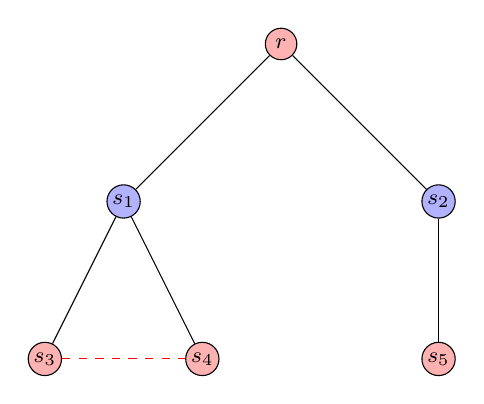
\begin{tikzpicture}[scale=1, every node/.style={circle, draw, fill=blue!20, inner sep=1pt, font=\footnotesize, minimum size=4mm}]
            \node[fill=red!30] (r) at (0, 0) {\(r\)};
            \node[fill=blue!30] (s1) at (-2, -2) {\(s_1\)};
            \node[fill=blue!30] (s2) at (2, -2) {\(s_2\)};

            \node[fill=red!30] (s3) at (-3, -4) {\(s_3\)};
            \node[fill=red!30] (s4) at (-1, -4) {\(s_4\)};
            \node[fill=red!30] (s5) at (2, -4) {\(s_5\)};

            \draw (r) -- (s1);
            \draw (r) -- (s2);

            \draw (s1) -- (s3);
            \draw (s1) -- (s4);
            \draw (s2) -- (s5);

            \draw[red, dashed] (s3) -- (s4);
        \end{tikzpicture}
    }
}